\chapter{\protect Introduction}
\label{introduction}

According to Hindu cosmological mythology, ancient people believe that a giant turtle bears the world on its back. Even after we stepped onto the moon at 1969, there are still plenty that we cannot explain. Recently, a group of scientists put a dilute NH$_4$CN in temperature of liquid nitrogen for 27 years and discovered a wide variaty of pyrimidine and purines \cite{miyakawa2002cold}. NH$_4^+$CN$^-$ plays an important role in life evolution. The formation of CN$^-$ is proposed by Kim and Kaiser (2001) \cite{kim},which is produced by ammonia (NH$_3$) and methane (CH$_4$). However, they have only demonstrated the effects of energetic electrons onto the ice mixtures, the photolysis experiments of CH$_4$+NH$_3$ ice mixtures especially variating relative proportions of CH$_4$ to NH$_3$ by VUV or EUV photons has not been performed. This thesis aims to investigate the chemistry of VUV and EUV irradiations on CH$_4$+NH$_3$ ice mixtures, which is possibly one of the main starting components to form CN$^-$ in astrophysical environments.\\

NH$_3$ is often not probed in astrophysical environments unless detecting ambiguously because nearly all the infrared bands overlap with water. The "unbrella" mode (1070 cm$^{-1}$) is often obscured by the 10 micron silicate feature \cite{d1986time}. It is often detected as ammonia hydrates (NH3 $\cdot$ nH$_2$O)\cite{cook2007near}. The New Horizons team has revealed a high concentration crater of NH$_3$ on Charon\cite{grundy2016surface}. Figure \ref{fig:Charon_IR} presents the infrared spectra detected by LEISA camera regarding four different segments at the right panel. On Organa crater, we may observe a 2.2 $\mu$m absorption representing presence of ammonia at "b" spectrum. The part b spectrum is enlarged at left bottom panel with the green pigments indicates the concentration of ammonia overlapped on topological graph of Charon. This also explains the different concentration of ammonia detected by different earth-based observation groups cook et al (2007)\cite{cook2007near} and brown et al. (2000)\cite{brown2000evidence}.\\

Charon, as a member in the Pluto system, is the second massive member with masses about half of Pluto. It orbits around Pluto, where Pluto is orbiting the Sun with an semi-major axis of 39.1 A.U. and period of 248 earth years. Similar to the earth and moon system, they orbits synchronized to each other with tidal-lockings, which the same side always facing each other. CH$_4$ is the main ejecta arrived from Pluto to Charon (98 \% by calculation of Hoey et al. (2017)\cite{hoey2017rarefied}. According to the New Horizons team, CH$_4$ from Pluto may accumulate onto the surface of Charon by cold-trapping which deposits at temperature below 25 K (at pressure $7.4 \times 10^{-14}$ torr) onto the surface of Charon\cite{grundy2016formation}. The amount of CH$_4$ varies along the surface of Charon because it depends on the length of time the temperature is below 25 K which in turns depends on diurnal motion and thermal inertia of Charon. With obliquity of 119 degrees (currently) from the ecliptic, a long continuous darkness is expected. The upper panel of Figure \ref{fig:Charon_thermal} is the model simulated by Grundy et al. (2016)\cite{grundy2016formation} presenting the surface temperature of Charon with respect to the lattitude and time in earth years. Based on length of time the surface temperature falls below 25 K, he plotted the length of time that CH$_4$ can accumulate onto Charon at the lower panel. From bottom panel, the mean cold-trap longitivity for depositing CH$_4$ is 2 times longer at the poles (130 earth years) than at 45$^{\circ}$ lattitude \cite{grundy2016formation}.The non-detection of methane by infrared spectra implies that its concentration is less than ammonia. However, the exact concentration ratios to ammonia was not fully modelled yet. Therefore, we decided to perform 3 relative ratios of CH$_4$ to NH$_3$ (in excess) to simulate the surface of Charon. They includes CH$_4$ to NH$_3$ equals 1:5, 1:10 and 1:20.\\

\begin{figure}
\centering
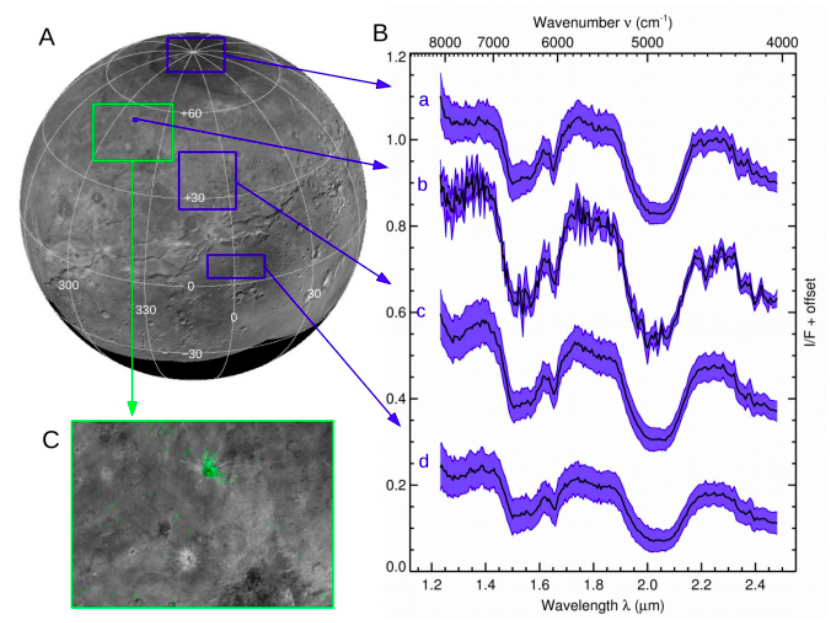
\includegraphics[width=\textwidth]{figures/chapter1/IR.png}
\caption{The 2.2$\mu$m absorption taken by LEISA camera colored as green on the topology shown by LORRI camera (A) and the spectra at 4 positions (B) with b taken near organa crater.(quoted from \cite{grundy2016surface})}
\label{fig:Charon_IR}
\end{figure}

Despite methane and ammonia, we still need energy to generate CN$^-$. In our solar system, there are many energetic sources, including solar wind, photons, cosmic rays from the outer solar system, etc. Among these, Ly-$\alpha$ photons appears to be the most important source in the dark side of Charon. It is attributed from sunlit(70 \%) and resonance scattering by atomic hydrogen flow (the excitment of electrons by hydrogen atoms and release ly-$\alpha$ photons in all directions)(30 \%) in the solar system \cite{grundy2016formation}. Its flux is $3.5 \times 10^7$ photons cm$^{-2}$ s$^{-1}$ at the winter pole of Charon \cite{grundy2016formation} which is 50 \% larger than expected before Mission New Horizons \cite{gladstone2015lyalpha}. We perform VUV irradiation on CH$_4$+NH$_3$ experiments with different ratios (including 3:2, 1:5, 1:10 and 1:20) to simulate the photon induced evolution on different concentrations of CH$_4$. The ratios in previous studies with electron irradiation experiments are CH$_4$ to NH$_3$ equals 3:1\cite{kim} and 3:2\cite{kundu2017electron}. As a complete study, we decided performing a ratio of CH$_4$ to NH$_3$ equals 3:2 to make possible comparisons.

\begin{figure}
\centering
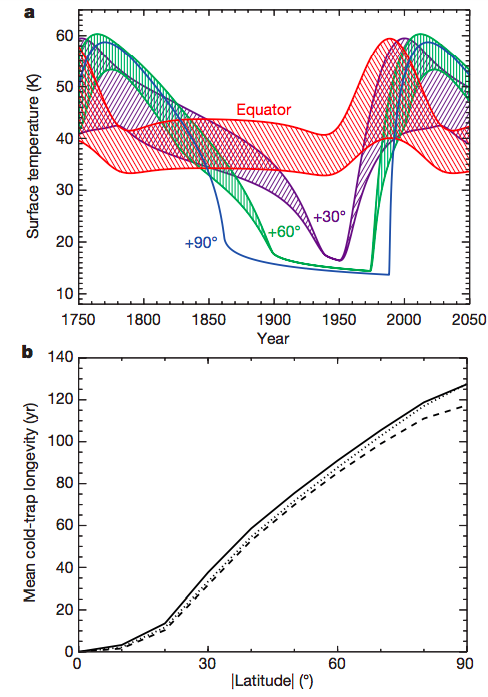
\includegraphics[width=0.5\textwidth]{figures/chapter1/thermal.png}
\caption{The temperature of Charon with thermal inertia 10 J m$^{-2}$ K$^{-1}$ s$^{-1/2}$ in 1750 to 2050 Earth years (a) and longest time the Latitude is under 25 K with the model averaged for 3 Myr with 2.5 (solid) 10 (dotted) and 40 (dashed) J m$^{-2}$ K$^{-1}$ s$^{-1/2}$ (b).(quoted from \cite{grundy2016formation})}
\label{fig:Charon_thermal}
\end{figure}

Apart from VUV irradiation, EUV irradiation also irradiates on Charon. The direct EUV irradiation (>12.4 eV) is $8.7 \times 10^7$ eV cm$^{-2}$ s$^{-1}$ at mean heliocentric distance 39 A.U. whereas VUV irradiation (Ly-$\alpha$ photons) is $1.9 \times 10^9$ eV cm$^{-2}$ s$^{-1}$ calculated by Grundy et al. (2016)\cite{grundy2016formation}. In order to investigate the effectiveness of EUV to VUV irradiation, we keep temperature of CH$_4$+NH$_3$ (3:2 \& 1:5) ice mixtures at 15 K and use the monochromatic 30.4 nm (40.8 eV) ,He II light provided by High flux beamline at National Synchrotron Radiation Research Centre (NSRRC) in Taiwan to irradiate the ice mixtures. The relative ratios of EUV irradiated ice is CH$_4$ to NH$_3$ = 3:2 and 1:5 for possible comparisons with VUV irradiations. \\

In this text, we will introduce the experimental methodology in chapter \ref{methods}, the formation mechanisms of main products of  EUV and VUV irradiated CH$_4$+NH$_3$ ice mixtures in chapter \ref{results}. With these results, we will know more details of Charon, especially the influences of photon sources. Different energy sources including electron irradiation experiments , EUV and VUV irradiations, and their astrophysical implications will be presented in chapter \ref{astron}.\\
